% ============================================================
%  SECTION 1 — BACKGROUND & MOTIVATION
% ============================================================

\begin{frame}{Background: Elastic Energy Storage}
  \begin{columns}[T]
    \column{0.55\textwidth}
    \begin{itemize}
      \item Planar elastic structures store energy through
            reversible deformation under load.
      \item Applications: compliant mechanisms, MEMS actuators,
            soft robotic grippers, mechanical springs
            \cite{howell2001}.
      \item Key metric: \textbf{energy storage efficiency}
            \[
              \eta = \frac{E_{\text{out}}}{E_{\text{in}}}
              = \frac{\int F_{\text{out}}\,\dd{x}}
                     {\int F_{\text{in}}\,\dd{x}}
            \]
    \end{itemize}

    \column{0.42\textwidth}
    % Conceptual figure: elastic beam stores energy
    \centering
    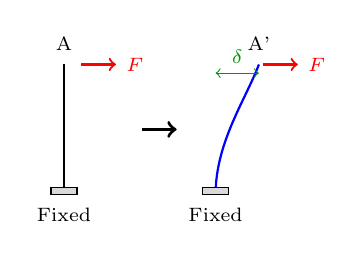
\begin{tikzpicture}[scale=0.55, every node/.style={font=\scriptsize}]
      % Undeformed
      \draw[thick] (0,0) -- (0,3);
      \draw[fill=gray!30] (-0.3,0) rectangle (0.3,0.15);
      \node[below] at (0,-0.1) {Fixed};
      \draw[->,red,thick] (0.4,3) -- (1.2,3) node[right]{$F$};
      \node[above] at (0,3.1) {A};

      % Arrow
      \draw[->,very thick] (1.8,1.5) -- (2.6,1.5);

      % Deformed
      \draw[thick, blue] (3.5,0) .. controls (3.5,1.2) and (4.2,2.2) .. (4.5,3);
      \draw[fill=gray!30] (3.2,0) rectangle (3.8,0.15);
      \node[below] at (3.5,-0.1) {Fixed};
      \draw[->,red,thick] (4.6,3) -- (5.4,3) node[right]{$F$};
      \node[above] at (4.5,3.1) {A'};
      \draw[<->,green!60!black] (3.5,2.8) -- (4.5,2.8)
            node[midway,above]{$\delta$};
    \end{tikzpicture}
  \end{columns}
\end{frame}

\begin{frame}{Topology Optimization for Structures}
  \small
  \begin{columns}[T]
    \column{0.58\textwidth}
    \begin{itemize}\setlength\itemsep{2pt}
      \item \textbf{Topology optimization}: find optimal material
            layout in a fixed domain \cite{bendsoe2003topology}.
      \item SIMP method: density $\rho_e \in [0,1]$ per element
            \cite{sigmund2001}.
      \item Applied in aerospace, automotive, biomedical
            \cite{liu2018topology}.
      \item \textbf{Gap:} few studies experimentally validate
            topology-optimised planar energy-storing structures
            \cite{zhu2020compliant, tong2023spring}.
    \end{itemize}

    \column{0.40\textwidth}
    \centering
    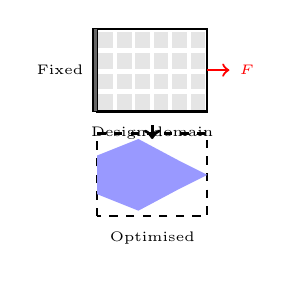
\begin{tikzpicture}[scale=0.35, every node/.style={font=\tiny}]
      % Design domain
      \draw[thick] (0,0) rectangle (4,3);
      \foreach \x in {0,0.67,...,3.5}{
        \foreach \y in {0,0.75,...,2.5}{
          \fill[gray!20] (\x+0.05,\y+0.05) rectangle (\x+0.58,\y+0.62);
        }
      }
      \node[below] at (2,-0.2) {Design domain};
      \draw[fill=black!60] (-0.15,0) rectangle (0,3);
      \node[left] at (-0.15,1.5) {Fixed};
      \draw[->,red,thick] (4,1.5) -- (4.8,1.5) node[right]{$F$};

      \draw[->,very thick] (2,-0.5) -- (2,-1.0);

      \begin{scope}[yshift=-3.8cm]
        \draw[thick,dashed] (0,0) rectangle (4,3);
        \fill[blue!40] (0,2.2) -- (1.5,2.8) -- (3,2) -- (4,1.5)
                        -- (3,1) -- (1.5,0.2) -- (0,0.8) -- cycle;
        \fill[blue!40] (0,1.2) -- (1,1.5) -- (2,1.5) -- (0,1.8) -- cycle;
        \node[below] at (2,-0.2) {Optimised};
      \end{scope}
    \end{tikzpicture}
  \end{columns}
\end{frame}
